\documentclass[a4paper]{article}

\usepackage[UTF8]{ctex}
\usepackage[a4paper,margin=1in]{geometry}
\usepackage{amsmath} % Ensure amsmath package is included to support mathematical formulas
\usepackage{graphicx}
\usepackage{float}
\usepackage{listings}
\usepackage{longtable}
\usepackage{booktabs}
\usepackage{hyperref}
\usepackage{fancyhdr}
\usepackage{lastpage}
\usepackage{color}
\usepackage{indentfirst}        % First paragraph indentation
\setlength{\parindent}{2em}     % Indent 2 characters
\usepackage{zhnumber}           % Chinese numbering
\usepackage[dvipsnames]{xcolor}

%\newcommand{\college}{School of Computer Science, Sun Yat-sen University}
\newcommand{\projname}{软件工程}
\newcommand{\reporttitle}{Python开源项目分析与CASE工具应用实践} % Update report title
\newcommand{\stuno}{23336179}
\newcommand{\authorname}{马福泉}
\newcommand{\major}{计算机科学与技术}
\newcommand{\adviser}{郑贵锋}
\newcommand{\labdate}{2025年6月}

\pagestyle{fancy} % Use fancyhdr style
\fancyhf{}      % Clear default headers and footers

% Set headers
\fancyhead[L]{\kaishu \projname}      % Left header shows project name
\fancyhead[C]{\kaishu \reporttitle}    % Center header shows report title (automatically uses updated title)
\fancyhead[R]{\kaishu \authorname} % Right header shows author name

% Set footers
\fancyfoot[C]{第 \thepage 页,共 17页} % Dynamic total pages

% Remove separator lines between headers/footers and content
\renewcommand{\headrulewidth}{0.4pt}
\renewcommand{\footrulewidth}{0pt}

% Set document background color
\definecolor{mybgcolor}{RGB}{0, 0, 0} % Define background color
\definecolor{NavyBlue}{RGB}{0,0,128} % Add color definition
% \pagecolor{mybgcolor} % Set background color

% Set listings style (if custom styling is needed)
\lstdefinestyle{pythoncode}{
    language=Python,
    basicstyle=\ttfamily\small,
    keywordstyle=\color{blue},
    commentstyle=\color{gray},
    stringstyle=\color{red},
    numbers=left,
    numberstyle=\tiny\color{gray},
    stepnumber=1,
    numbersep=5pt,
    backgroundcolor=\color{white}, % Set background color
    showspaces=false,
    showstringspaces=false,
    showtabs=false,
    frame=single, % Add border
    rulecolor=\color{black},
    tabsize=4,
    captionpos=b,
    breaklines=true,
    breakatwhitespace=false,
    title=\lstname,
    escapeinside={\%*}{*)}
}

\begin{document}

% Cover page
\begin{titlepage}
    \centering
    
\includegraphics[width=10cm]{img/SYSULogo.png}
    \vspace{1em}
    %{\Large \college \par}
    \vspace{1em}
    {\Large \kaishu \projname \par}
    \vspace{3em}
    {\fontsize{40pt}{42pt}\kaishu \selectfont \boldmath \reporttitle\par} % Cover title will also be automatically updated
    \vspace*{\fill}
    \begin{center}
    {\Large
    \makebox[5em][s]{学号}:\underline{\makebox[15em][c]{\kaishu \stuno}}\\[1em]
    \makebox[5em][s]{姓名}:\underline{\makebox[15em][c]{\kaishu \authorname}}\\[1em]
    \makebox[5em][s]{专业}:\underline{\makebox[15em][c]{\kaishu \major}}\\[1em]
    \makebox[5em][s]{任课教师}:\underline{\makebox[15em][c]{\kaishu \adviser}}\\[1em]
    \makebox[5em][s]{日期}:\underline{\makebox[15em][c]{\kaishu \labdate}}\\[1em]
    }
    \end{center}
    \vspace*{\fill}
\end{titlepage}

\begin{abstract}
本实践基于Snake Game和Todo App两个Python项目,深入探讨了CASE工具在软件工程实践中的应用。通过对这两个项目的深度代码分析,运用PlantUML、Pyreverse等CASE工具生成了完整的UML图表集,包括用例图、类图、时序图、状态图和活动图。实践过程涵盖了从环境搭建、代码分析到UML建模的完整流程,展示了现代软件工程中CASE工具的有效使用方法。通过对比分析游戏类应用和数据管理应用的不同设计模式,加深了对软件架构设计的理解。

\vspace{1em} % Add some vertical space between abstract and keywords
\noindent\textbf{关键词:} Snake Game;Todo App;CASE工具;UML建模;PlantUML;软件工程实践;代码分析;软件架构
\end{abstract}

\section{项目背景}

在现代软件开发中,UML(统一建模语言)作为软件系统设计的标准工具,对于理解和维护复杂软件系统具有重要意义。CASE(Computer-Aided Software Engineering)工具的出现,使得UML建模过程更加高效和标准化。

\begin{figure}[H]
\centering

\includegraphics[width=\textwidth]{img/1.png}
\caption{项目背景}
\label{fig:project_overview}
\end{figure}

本项目选择了两个具有代表性的Python应用进行深入分析:Snake Game(贪吃蛇游戏)和Todo App(待办事项应用)。这两个项目分别代表了实时交互游戏和数据管理应用的典型特征,通过对比分析能够全面理解不同类型软件的设计思路和架构模式。

软件工程的核心理念是通过系统化、规范化的方法来开发和维护软件系统。在这一过程中,设计文档和架构图表起到了至关重要的作用,它们不仅帮助开发者理解系统结构,还为后续的维护和扩展提供了重要参考。

\section{作业介绍}

本次实践作业旨在通过实际的Python项目,掌握CASE工具的使用方法和UML建模技术。作业内容包括以下几个核心部分:

\subsection{实践目标}

\begin{itemize}
    \item \textbf{环境搭建}:在Windows系统上完整搭建CASE工具开发环境,包括Java、Python、PlantUML、Graphviz等工具的安装配置
    \item \textbf{代码分析}:深入分析Snake Game和Todo App两个项目的代码结构、算法实现和设计模式
    \item \textbf{UML建模}:运用PlantUML等工具生成完整的UML图表集,包括用例图、类图、时序图、状态图和活动图
    \item \textbf{工具实践}:掌握多种CASE工具的使用方法,包括手工建模和自动分析工具
    \item \textbf{对比分析}:通过两个不同类型项目的对比,理解不同软件架构的设计思路
\end{itemize}

\subsection{技术栈和工具链}

本实践采用了完整的现代软件工程工具链:

\begin{itemize}
    \item \textbf{开发语言}:Python 3.11+
    \item \textbf{建模工具}:PlantUML、Visual Paradigm Community
    \item \textbf{自动分析工具}:Pyreverse(Pylint的组件)
    \item \textbf{辅助工具}:Graphviz、Java 11+
    \item \textbf{开发环境}:Visual Studio Code + PlantUML扩展
    \item \textbf{版本控制}:完整的文档和代码管理
\end{itemize}

\subsection{实践方法论}

本实践采用了逆向工程的方法论,即从现有代码出发,通过分析和理解来生成设计文档:

\begin{enumerate}
    \item \textbf{代码理解阶段}:深入阅读和分析现有Python代码,理解其功能实现和设计思路
    \item \textbf{结构抽象阶段}:从代码中抽象出类关系、交互模式和业务流程
    \item \textbf{模型构建阶段}:使用UML标准语言描述系统的静态结构和动态行为
    \item \textbf{工具实践阶段}:运用多种CASE工具实现建模过程的自动化
    \item \textbf{验证完善阶段}:通过多种方法验证模型的正确性和完整性
\end{enumerate}

这种方法不仅有助于理解现有系统,更重要的是培养了从代码到设计的抽象思维能力。

\section{Python代码介绍}

基于对Snake Game和Todo App两个项目的深入分析,本节将详细介绍它们的代码结构、核心算法和设计特点。

\subsection{Snake Game项目分析}

Snake Game是一个基于Tkinter的经典贪吃蛇游戏,体现了实时交互游戏的典型架构模式。

\subsubsection{项目结构}

Snake Game采用单文件架构,所有逻辑集中在\texttt{snake\_game.py}文件中:


\subsubsection{核心类设计}

\textbf{Snake类设计}

Snake类负责管理蛇的状态和行为,采用了坐标列表和视觉元素分离的设计:

\begin{lstlisting}[style=pythoncode, caption=Snake类核心代码]
class Snake:
    def __init__(self):
        self.body_size = BODY_PARTS
        self.coordinates = []  # Store coordinates of each part of snake body
        self.squares = []      # Store graphic elements on canvas
        
        # Initialize snake body coordinates (starting from head)
        for i in range(0, BODY_PARTS):
            self.coordinates.append([0, 0])
        
        # Create visual elements of snake body on canvas
        for x, y in self.coordinates:
            square = canvas.create_rectangle(x, y, x + SPACE_SIZE, y + SPACE_SIZE, 
                                           fill=SNAKE_COLOR, tag="snake")
            self.squares.append(square)
\end{lstlisting}

\textbf{Food类设计}

Food类实现了食物的随机生成和网格对齐算法:

\begin{lstlisting}[style=pythoncode, caption=Food类核心代码]
class Food:
    def __init__(self):
        # Grid-aligned random position generation algorithm
        x = random.randint(0, (GAME_WIDTH / SPACE_SIZE)-1) * SPACE_SIZE
        y = random.randint(0, (GAME_HEIGHT / SPACE_SIZE) - 1) * SPACE_SIZE
        
        self.coordinates = [x, y]
        
        # Create circular food
        canvas.create_oval(x, y, x + SPACE_SIZE, y + SPACE_SIZE, 
                          fill=FOOD_COLOR, tag="food")
\end{lstlisting}

\subsubsection{核心算法分析}

\textbf{游戏主循环算法}

游戏主循环采用了递归调用的方式实现连续的游戏状态更新:

\begin{lstlisting}[style=pythoncode, caption=游戏主循环算法]
def next_turn(snake, food):
    x, y = snake.coordinates[0]
    
    # Calculate new head position based on direction
    if direction == "up":
        y -= SPACE_SIZE
    elif direction == "down":
        y += SPACE_SIZE
    elif direction == "left":
        x -= SPACE_SIZE
    elif direction == "right":
        x += SPACE_SIZE
    
    # Update snake body
    snake.coordinates.insert(0, (x, y))
    square = canvas.create_rectangle(x, y, x + SPACE_SIZE, y + SPACE_SIZE, 
                                   fill=SNAKE_COLOR)
    snake.squares.insert(0, square)
    
    # Food collision detection and handling
    if x == food.coordinates[0] and y == food.coordinates[1]:
        global score
        score += 1
        label.config(text="Score:{}".format(score))
        canvas.delete("food")
        food = Food()
    else:
        # If no food consumed, remove tail
        del snake.coordinates[-1]
        canvas.delete(snake.squares[-1])
        del snake.squares[-1]
    
    # Collision detection and recursive call
    if check_collisions(snake):
        game_over()
    else:
        window.after(SPEED, next_turn, snake, food)
\end{lstlisting}

\textbf{碰撞检测算法}

碰撞检测算法分为边界碰撞和自身碰撞两个部分,采用了优化的检测策略:

\begin{lstlisting}[style=pythoncode, caption=碰撞检测算法]
def check_collisions(snake):
    x, y = snake.coordinates[0]
    
    # Boundary collision detection (O(1) complexity)
    if x < 0 or x >= GAME_WIDTH:
        return True
    elif y < 0 or y >= GAME_HEIGHT:
        return True
    
    # Self collision detection (O(n) complexity, n is snake body length)
    for body_part in snake.coordinates[1:]:
        if x == body_part[0] and y == body_part[1]:
            return True
    
    return False
\end{lstlisting}

\subsection{Todo App项目分析}

Todo App是一个基于Flask的Web应用,展示了典型的数据管理应用架构。

\subsubsection{项目结构}

Todo App采用了Flask的标准目录结构,实现了完整的MVC架构

\subsubsection{数据模型设计}

Todo类实现了完整的任务数据模型,采用SQLAlchemy ORM进行数据管理:

\begin{lstlisting}[style=pythoncode, caption=Todo数据模型]
class Todo(db.Model):
    id = db.Column(db.Integer, primary_key=True)
    content = db.Column(db.String(200), nullable=False)
    completed = db.Column(db.Integer, default=0)
    pub_date = db.Column(db.DateTime, nullable=False, default=datetime.utcnow)

    def __repr__(self):
        return "<Task %r>" % self.id
\end{lstlisting}

\subsubsection{核心功能实现}

\textbf{任务管理的CRUD操作}

应用实现了完整的任务管理功能,包括创建、读取、更新和删除:

\begin{lstlisting}[style=pythoncode, caption=任务管理核心逻辑]
@app.route("/", methods=["POST", "GET"])
def index():
    if request.method == "POST":
        task_content = request.form["task"]
        new_task = Todo(content=task_content)
        try:
            db.session.add(new_task)
            db.session.commit()
            return redirect("/")
        except:
            return "There is an issue"
    else:
        tasks = Todo.query.order_by(Todo.pub_date).all()
        return render_template("index.html", tasks=tasks)

@app.route("/delete/<int:id>")
def delete(id):
    task = Todo.query.get_or_404(id)
    try:
        db.session.delete(task)
        db.session.commit()
        return redirect("/")
    except:
        return "This is an Problem while deleting"
\end{lstlisting}

\subsection{项目对比分析}

通过对两个项目的深入分析,可以发现它们在架构设计上的显著差异:

\begin{table}[H]
\centering
\caption{Snake Game与Todo App对比分析}
\begin{tabular}{|l|l|l|}
\hline
\textbf{特性} & \textbf{Snake Game} & \textbf{Todo App} \\
\hline
架构模式 & 游戏循环 + MVC & 分层架构 + MVP \\
\hline
数据模型 & 实时状态管理 & 持久化数据存储 \\
\hline
用户交互 & 连续键盘输入 & 事件驱动表单提交 \\
\hline
时间特性 & 实时性要求高 & 异步处理 \\
\hline
状态管理 & 内存中的临时状态 & 数据库中的持久状态 \\
\hline
复杂度 & 算法复杂度:O(n) & 数据操作复杂度:O(1)-O(n) \\
\hline
\end{tabular}
\end{table}

这种对比分析有助于理解不同类型应用的设计原则和技术选择,为今后的软件开发提供了重要的参考价值。

\section{CASE工具使用介绍}

本节详细介绍了CASE工具在本项目中的应用,包括环境搭建、工具配置和UML建模的完整过程。

\subsection{CASE工具环境搭建}

为了确保UML建模工作的顺利进行,本项目建立了完整的CASE工具开发环境。

\subsubsection{核心工具链}

本项目采用的CASE工具链包括:

\begin{itemize}
    \item \textbf{PlantUML}:开源的UML图表生成工具,支持多种图表类型
    \item \textbf{Pyreverse}:Python专用的代码分析工具,能够自动生成类图
    \item \textbf{Graphviz}:图形渲染引擎,为PlantUML提供底层支持
    \item \textbf{Visual Studio Code}:集成开发环境,配合PlantUML扩展实现可视化建模
\end{itemize}

\subsubsection{环境配置过程}

完整的环境搭建过程包括以下步骤:

\begin{enumerate}
    \item \textbf{Java环境配置}:安装OpenJDK 11,配置JAVA\_HOME和PATH环境变量
    \item \textbf{Python环境准备}:安装Python 3.11+,通过pip安装pylint包
    \item \textbf{Graphviz安装}:下载并安装Graphviz,配置系统PATH
    \item \textbf{PlantUML配置}:下载plantuml.jar文件,验证工具链的完整性
    \item \textbf{开发环境集成}:在VS Code中安装PlantUML扩展,配置本地JAR路径
\end{enumerate}

通过批处理脚本实现了环境验证的自动化,确保所有工具能够正常协作。

\subsection{UML建模实践过程}

\subsubsection{建模方法论}

本项目采用了多层次的建模方法:

\begin{itemize}
    \item \textbf{手工建模}:使用PlantUML语法手工创建UML图表,确保模型的准确性和完整性
    \item \textbf{自动生成}:使用Pyreverse从源代码自动生成类图,作为手工建模的补充和验证
    \item \textbf{对比分析}:通过手工模型和自动生成模型的对比,发现设计中的潜在问题
\end{itemize}

\subsubsection{UML图表类型及其应用}

\textbf{用例图(Use Case Diagram)}

用例图展示了系统的功能需求和用户交互关系,是需求分析的重要工具。

\begin{figure}[H]
\centering
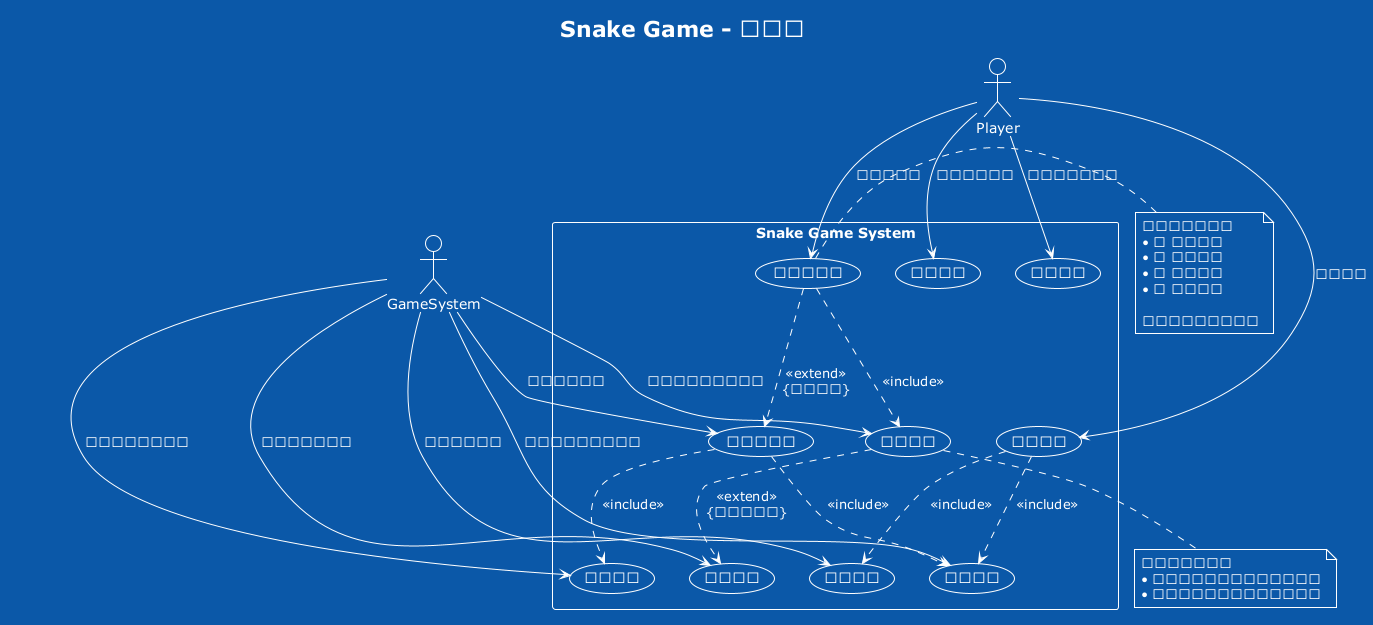
\includegraphics[width=\textwidth]{img/Snake_Game_UseCase.png}
\caption{Snake Game用例图}
\label{fig:snake_usecase}
\end{figure}

Snake Game的用例图清晰地展示了玩家与游戏系统的交互模式,包括基本的游戏控制、分数管理和游戏状态转换等核心功能。

\textbf{类图(Class Diagram)}

类图是面向对象设计的核心工具,展示了系统中类的结构和关系。

\begin{figure}[H]
\centering
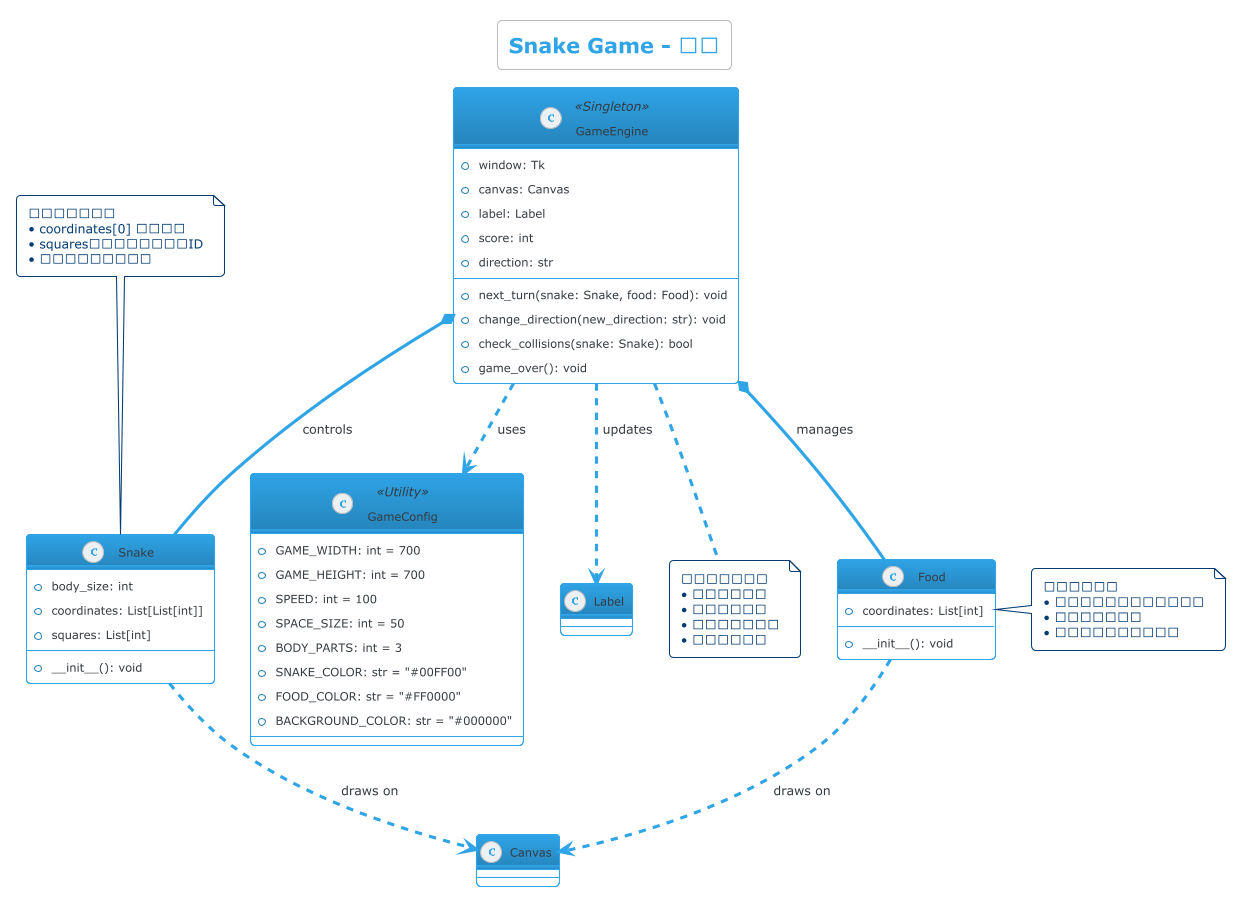
\includegraphics[width=\textwidth]{img/Snake_Game_Class.png}
\caption{Snake Game类图 - PlantUML手工建模}
\label{fig:snake_class_manual}
\end{figure}

\begin{figure}[H]
\centering
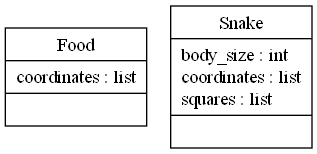
\includegraphics[width=\textwidth]{img/classes_SnakeGame_Auto.png}
\caption{Snake Game类图 - Pyreverse自动生成}
\label{fig:snake_class_auto}
\end{figure}

通过对比手工建模和自动生成的类图,可以发现手工模型更注重逻辑关系的表达,而自动生成的模型更接近实际的代码结构。

\textbf{时序图(Sequence Diagram)}

时序图描述了对象间的交互过程,特别适合表达复杂的业务流程。

\begin{figure}[H]
\centering
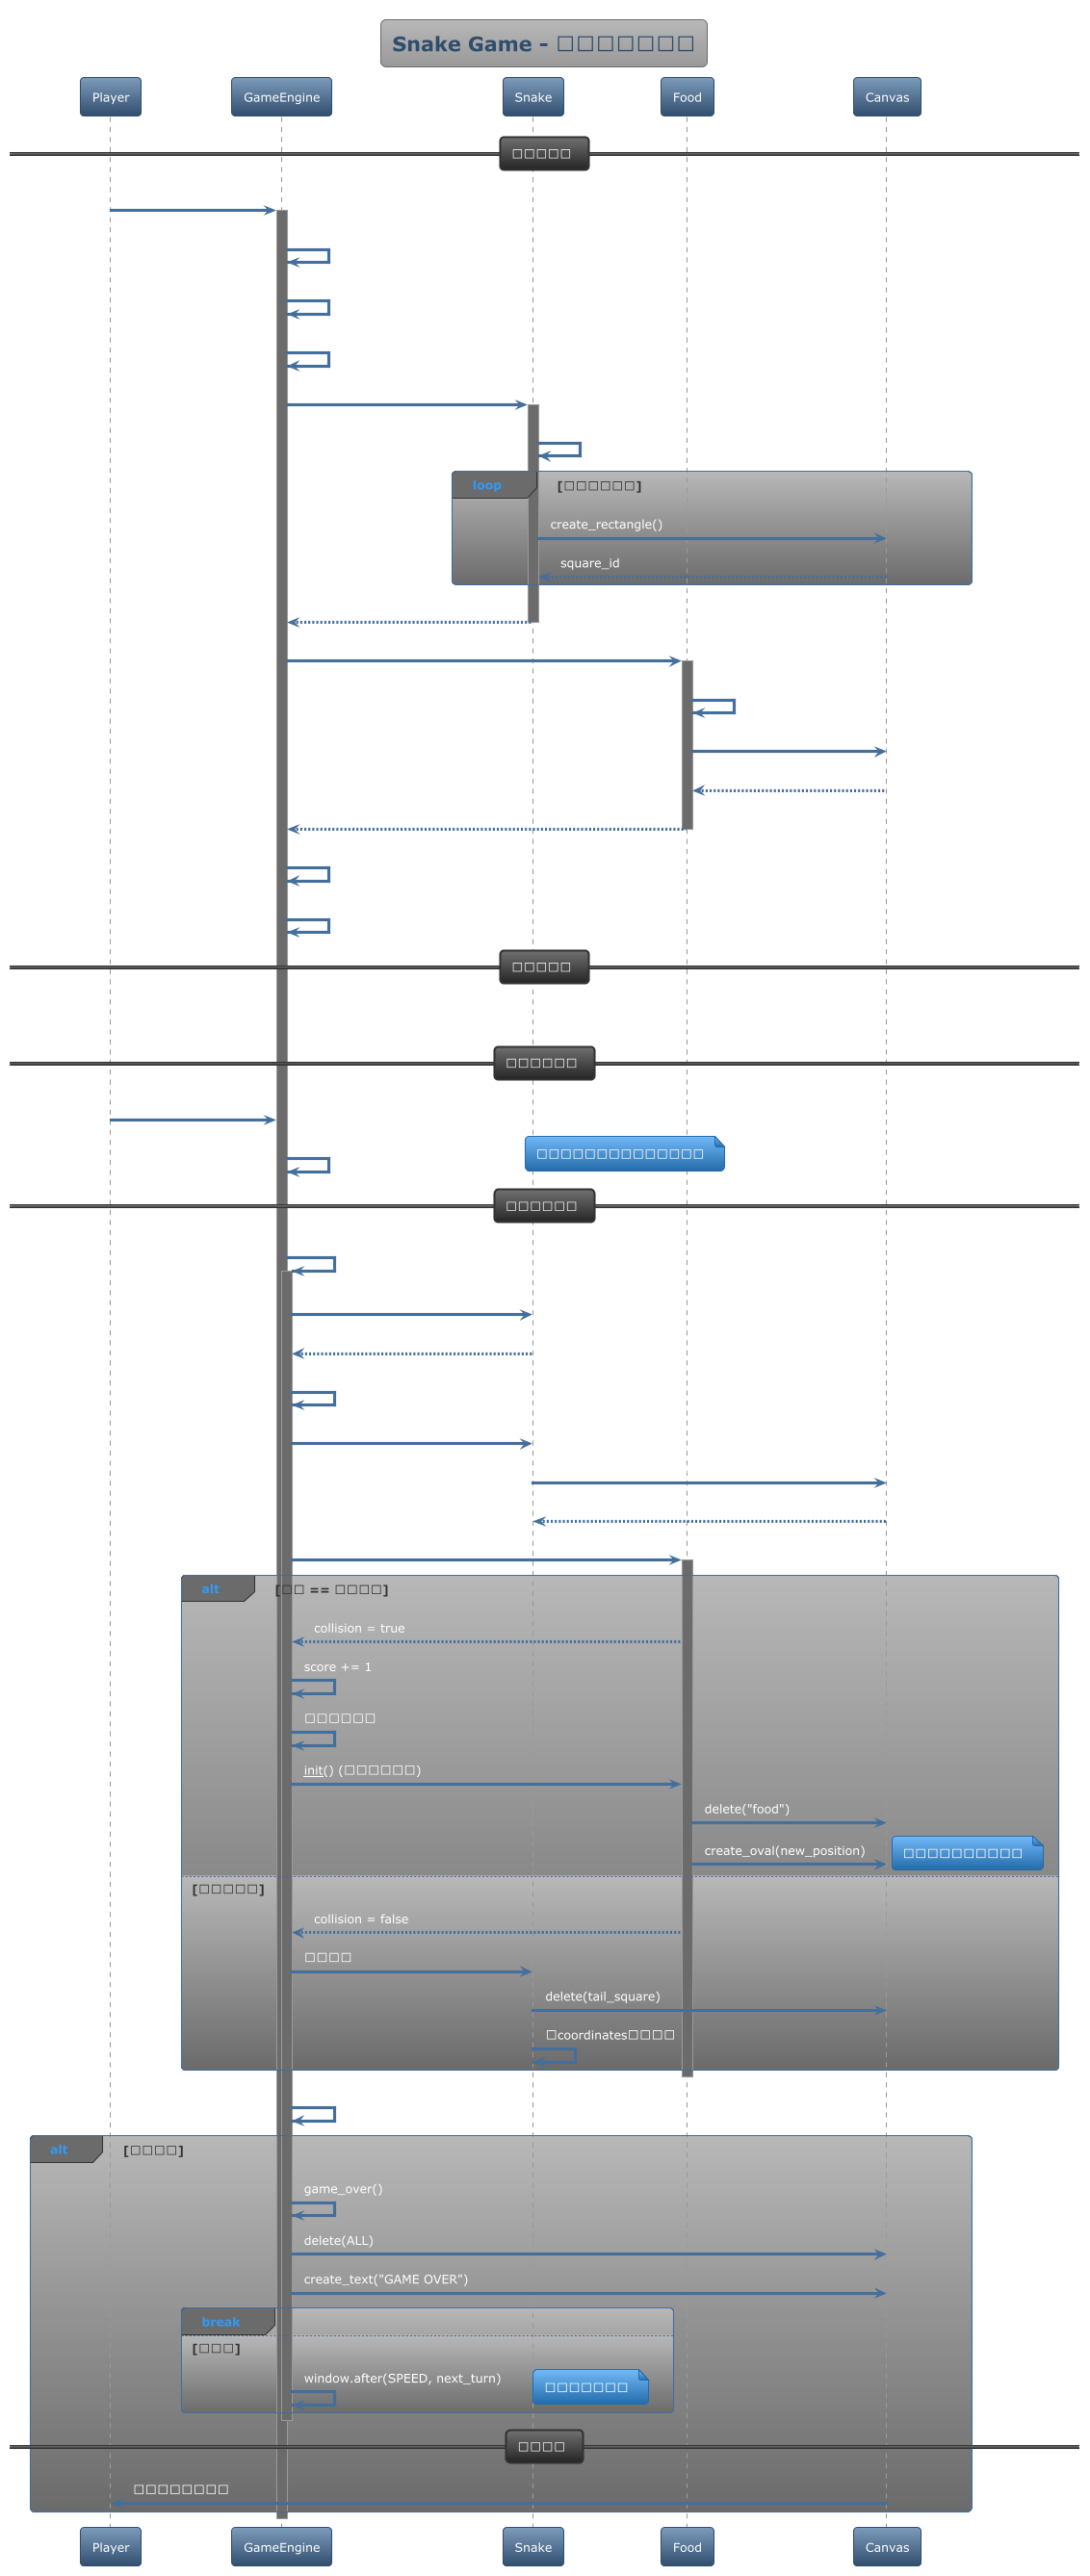
\includegraphics[width=\textwidth]{img/Snake_Game_Sequence.png}
\caption{Snake Game时序图 - 游戏循环过程}
\label{fig:snake_sequence}
\end{figure}

时序图详细展示了Snake Game中游戏循环的完整过程,从用户输入处理到画面更新的每个步骤都得到了清晰的表达。

\textbf{状态图(State Diagram)}

状态图表达了系统的状态转换逻辑,对于理解复杂的状态管理很有帮助。

\begin{figure}[H]
\centering
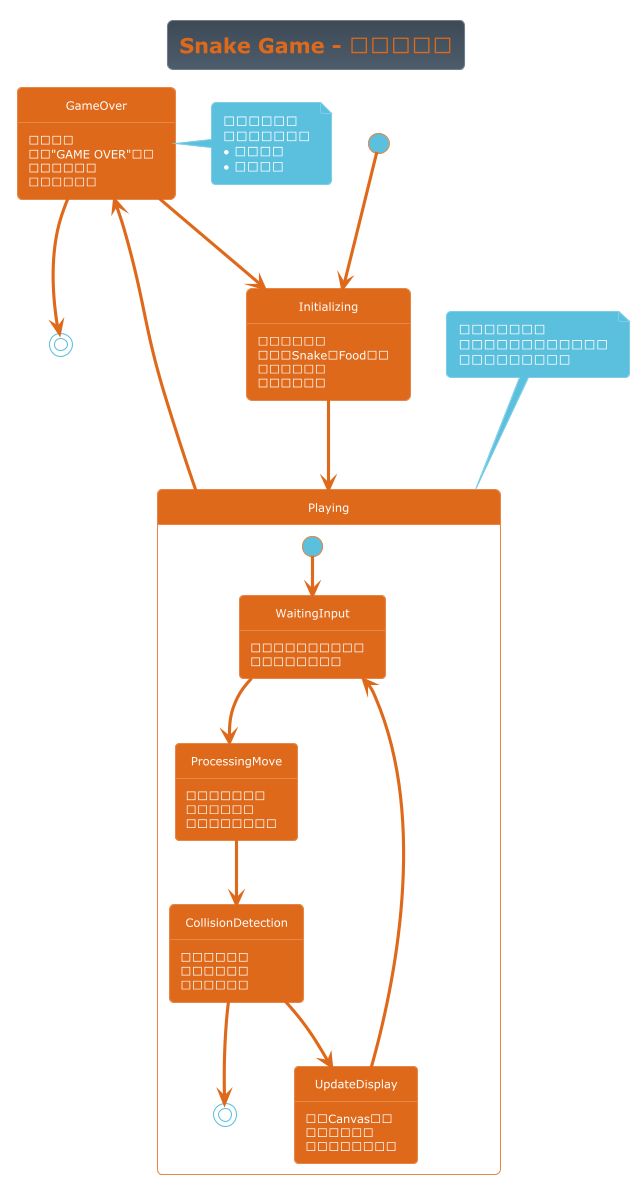
\includegraphics[width=\textwidth]{img/Snake_Game_State.png}
\caption{Snake Game状态图}
\label{fig:snake_state}
\end{figure}

\textbf{活动图(Activity Diagram)}

活动图展示了业务流程和算法逻辑,是过程建模的重要工具。

\begin{figure}[H]
\centering
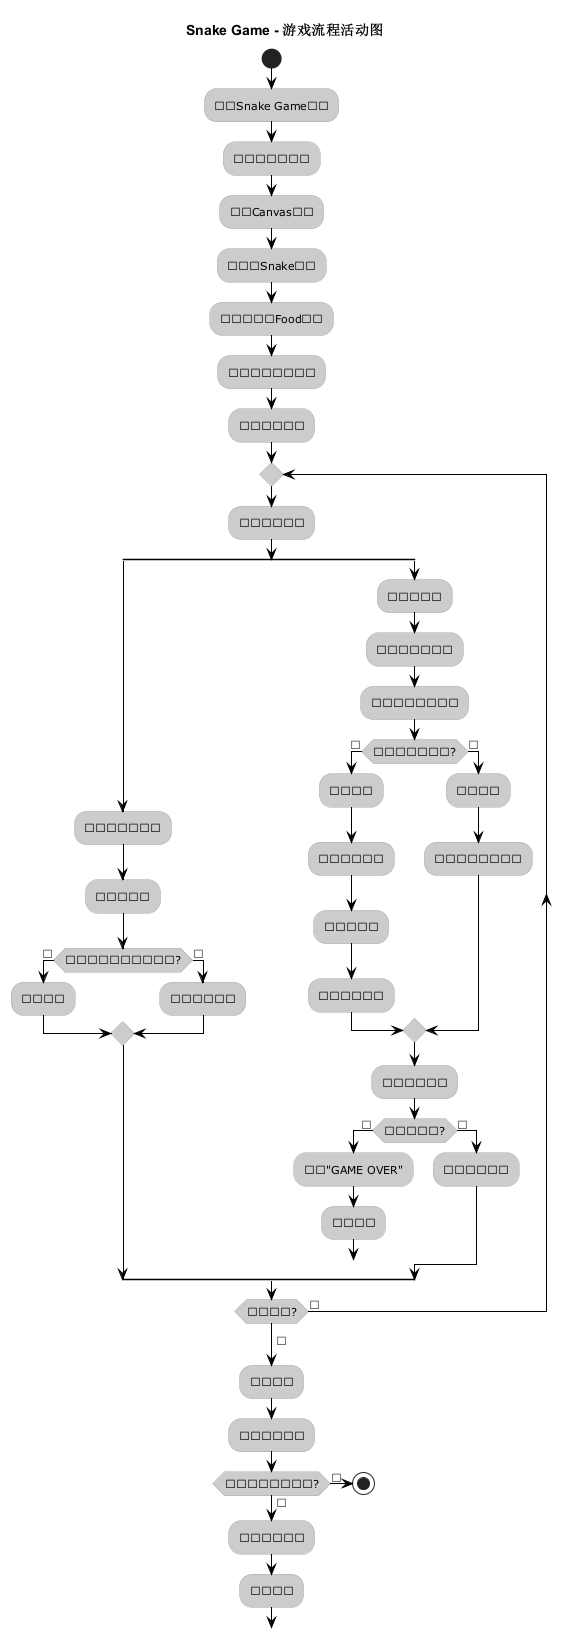
\includegraphics[width=\textwidth]{img/Snake_Game_Activity.png}
\caption{Snake Game活动图}
\label{fig:snake_activity}
\end{figure}

\subsection{建模工具的对比评估}

\subsubsection{PlantUML的优势}

\begin{itemize}
    \item \textbf{文本化建模}:使用简洁的文本语法,易于版本控制和协作
    \item \textbf{自动布局}:智能的图形布局算法,减少手工调整的工作量
    \item \textbf{多格式支持}:支持PNG、SVG、PDF等多种输出格式
    \item \textbf{开源免费}:完全开源,适合学习和研究使用
\end{itemize}

\subsubsection{Pyreverse的特点}

\begin{itemize}
    \item \textbf{代码分析}:直接从Python源代码生成类图,保证了模型与代码的一致性
    \item \textbf{自动化程度高}:无需手工建模,适合快速理解现有代码结构
    \item \textbf{依赖关系准确}:能够准确识别类之间的继承和依赖关系
\end{itemize}

\subsection{建模成果展示}

通过完整的建模过程,本项目生成了丰富的UML图表集:

\begin{table}[H]
\centering
\caption{生成的UML图表统计}
\begin{tabular}{|l|c|c|}
\hline
\textbf{图表类型} & \textbf{Snake Game} & \textbf{Todo App} \\
\hline
用例图 & ✓ & ✓ \\
\hline
类图(手工) & ✓ & ✓ \\
\hline
类图(自动) & ✓ & ✓ \\
\hline
时序图 & ✓ & ✓ \\
\hline
状态图 & ✓ & - \\
\hline
活动图 & ✓ & ✓ \\
\hline
\textbf{总计} & \textbf{6个} & \textbf{5个} \\
\hline
\end{tabular}
\end{table}

所有图表都采用了标准的UML语法和符号,确保了建模结果的专业性和可读性。同时,通过批处理脚本实现了图表生成的自动化,大大提高了建模效率。

这些UML图表不仅为理解现有系统提供了重要支撑,更为系统的后续维护和扩展奠定了坚实的文档基础。

\section{总结与心得体会}

通过本次Snake Game和Todo App项目的CASE工具UML建模实践,我深刻体会到了现代软件工程方法论的重要价值和实际应用效果。

\subsection{技术能力提升}

在本次实践中,我系统性地掌握了多项关键技能:

\subsubsection{CASE工具技能}
通过完整的环境搭建过程,我不仅学会了PlantUML、Pyreverse等工具的使用方法,更重要的是理解了工具链整合的重要性。从Java环境配置到Graphviz集成,每一个环节都需要细致的规划和验证。这个过程让我认识到,工具只是手段,关键在于建立系统化的工作流程。

\subsubsection{UML建模能力}
通过对两个不同类型项目的建模实践,我深入理解了UML各种图表的适用场景和表达能力。用例图帮助理清需求边界,类图揭示系统架构,时序图展现交互细节,状态图描述行为转换,活动图表达业务流程。每种图表都有其独特的价值,组合使用能够形成完整的系统视图。

\subsubsection{代码分析技能}
通过逆向工程的方式,从现有代码中抽象出设计模型,这个过程极大地提升了我的代码理解和分析能力。特别是在对比Snake Game的游戏循环模式和Todo App的MVC架构时,我深刻理解了不同应用领域对架构设计的不同要求。

\subsection{方法论认知}

\subsubsection{系统化思维}
本次实践让我认识到软件工程不仅仅是编写代码,更重要的是建立系统化的思维方式。从需求分析到架构设计,从代码实现到文档维护,每个环节都需要科学的方法和工具支撑。CASE工具正是这种系统化思维的体现,它将复杂的建模过程标准化、自动化,大大提高了开发效率。

\subsubsection{抽象能力}
通过UML建模,我学会了如何从具体的代码实现中抽象出通用的设计模式和架构原则。这种抽象能力不仅有助于理解现有系统,更为设计新系统提供了重要的思维工具。例如,通过分析Snake Game的碰撞检测算法,我理解了实时系统中性能优化的重要性;通过Todo App的数据模型设计,我掌握了关系型数据库在Web应用中的应用模式。

\subsubsection{对比分析方法}
通过同时分析两个不同类型的项目,我掌握了对比分析的方法论。这种方法不仅能够发现不同应用的共性特征,更能够深入理解特定领域的专业要求。游戏应用注重实时性和用户体验,数据应用关注一致性和可靠性,这些差异在UML模型中都得到了清晰的体现。

\subsection{实践价值体验}

\subsubsection{文档的重要性}
在建模过程中,我深刻体会到了高质量文档的价值。UML图表不仅是设计的产物,更是沟通的工具。清晰的类图能够帮助团队成员快速理解系统结构,详细的时序图能够指导测试用例的设计,完整的用例图能够确保需求的准确实现。

\subsubsection{工具与思维的关系}
通过使用多种CASE工具,我认识到工具本身只是辅助手段,真正重要的是背后的设计思维。PlantUML的文本化建模方式培养了结构化思维,Pyreverse的自动分析功能提高了工作效率,但最终的建模质量还是取决于对系统的深入理解和设计经验的积累。

\subsubsection{理论与实践的结合}
本次实践有效地将课堂上学到的软件工程理论与实际的项目开发结合起来。通过真实项目的建模过程,我不仅验证了理论知识的正确性,更重要的是学会了如何在实际工作中应用这些理论。这种理论与实践的结合,为今后的专业发展奠定了坚实基础。

\subsection{未来发展思考}

\subsubsection{技能扩展方向}
基于本次实践的收获,我认为未来需要在以下几个方向继续深化:
\begin{itemize}
    \item \textbf{架构设计能力}:学习更多的设计模式和架构风格,提升大型系统的设计能力
    \item \textbf{建模工具掌握}:探索更多的CASE工具,如Enterprise Architect、StarUML等商业化工具
    \item \textbf{敏捷建模方法}:学习如何在敏捷开发环境中有效地使用建模工具
    \item \textbf{领域特定建模}:针对不同的应用领域,掌握专门的建模方法和工具
\end{itemize}

\subsubsection{方法论深化}
在方法论层面,我希望能够:
\begin{itemize}
    \item \textbf{建立个人建模标准}:形成自己的建模风格和质量标准
    \item \textbf{提升抽象思维}:能够从更高层次思考系统架构和设计问题
    \item \textbf{培养系统思维}:将建模活动融入完整的软件开发生命周期
    \item \textbf{加强沟通能力}:使用建模成果进行有效的技术沟通
\end{itemize}

\subsection{总结感悟}

这次CASE工具UML建模实践是一次非常有价值的学习经历。它不仅让我掌握了实用的技术技能,更重要的是培养了系统化的软件工程思维。通过对Snake Game和Todo App两个项目的深入分析,我理解了不同类型软件的设计原则和技术选择,这为今后面对复杂软件系统提供了重要的方法论支撑。

软件工程是一门实践性很强的学科,理论知识只有通过实际项目的检验才能真正内化为能力。本次实践让我深刻体会到这一点,也激发了我继续深入学习软件工程理论和实践的热情。我相信,通过持续的学习和实践,一定能够在软件工程的道路上走得更远。

\end{document}